\chapter{Template float tests}
\label{appendix:test}
\acresetall

\section{Appendix introduction}

In this appendix we will test some float related packages used in this template and their settings.

\section{Test figure}

In \cref{figure:uml} we see an example of a figure.

\begin{figure}[htbp]
\centering
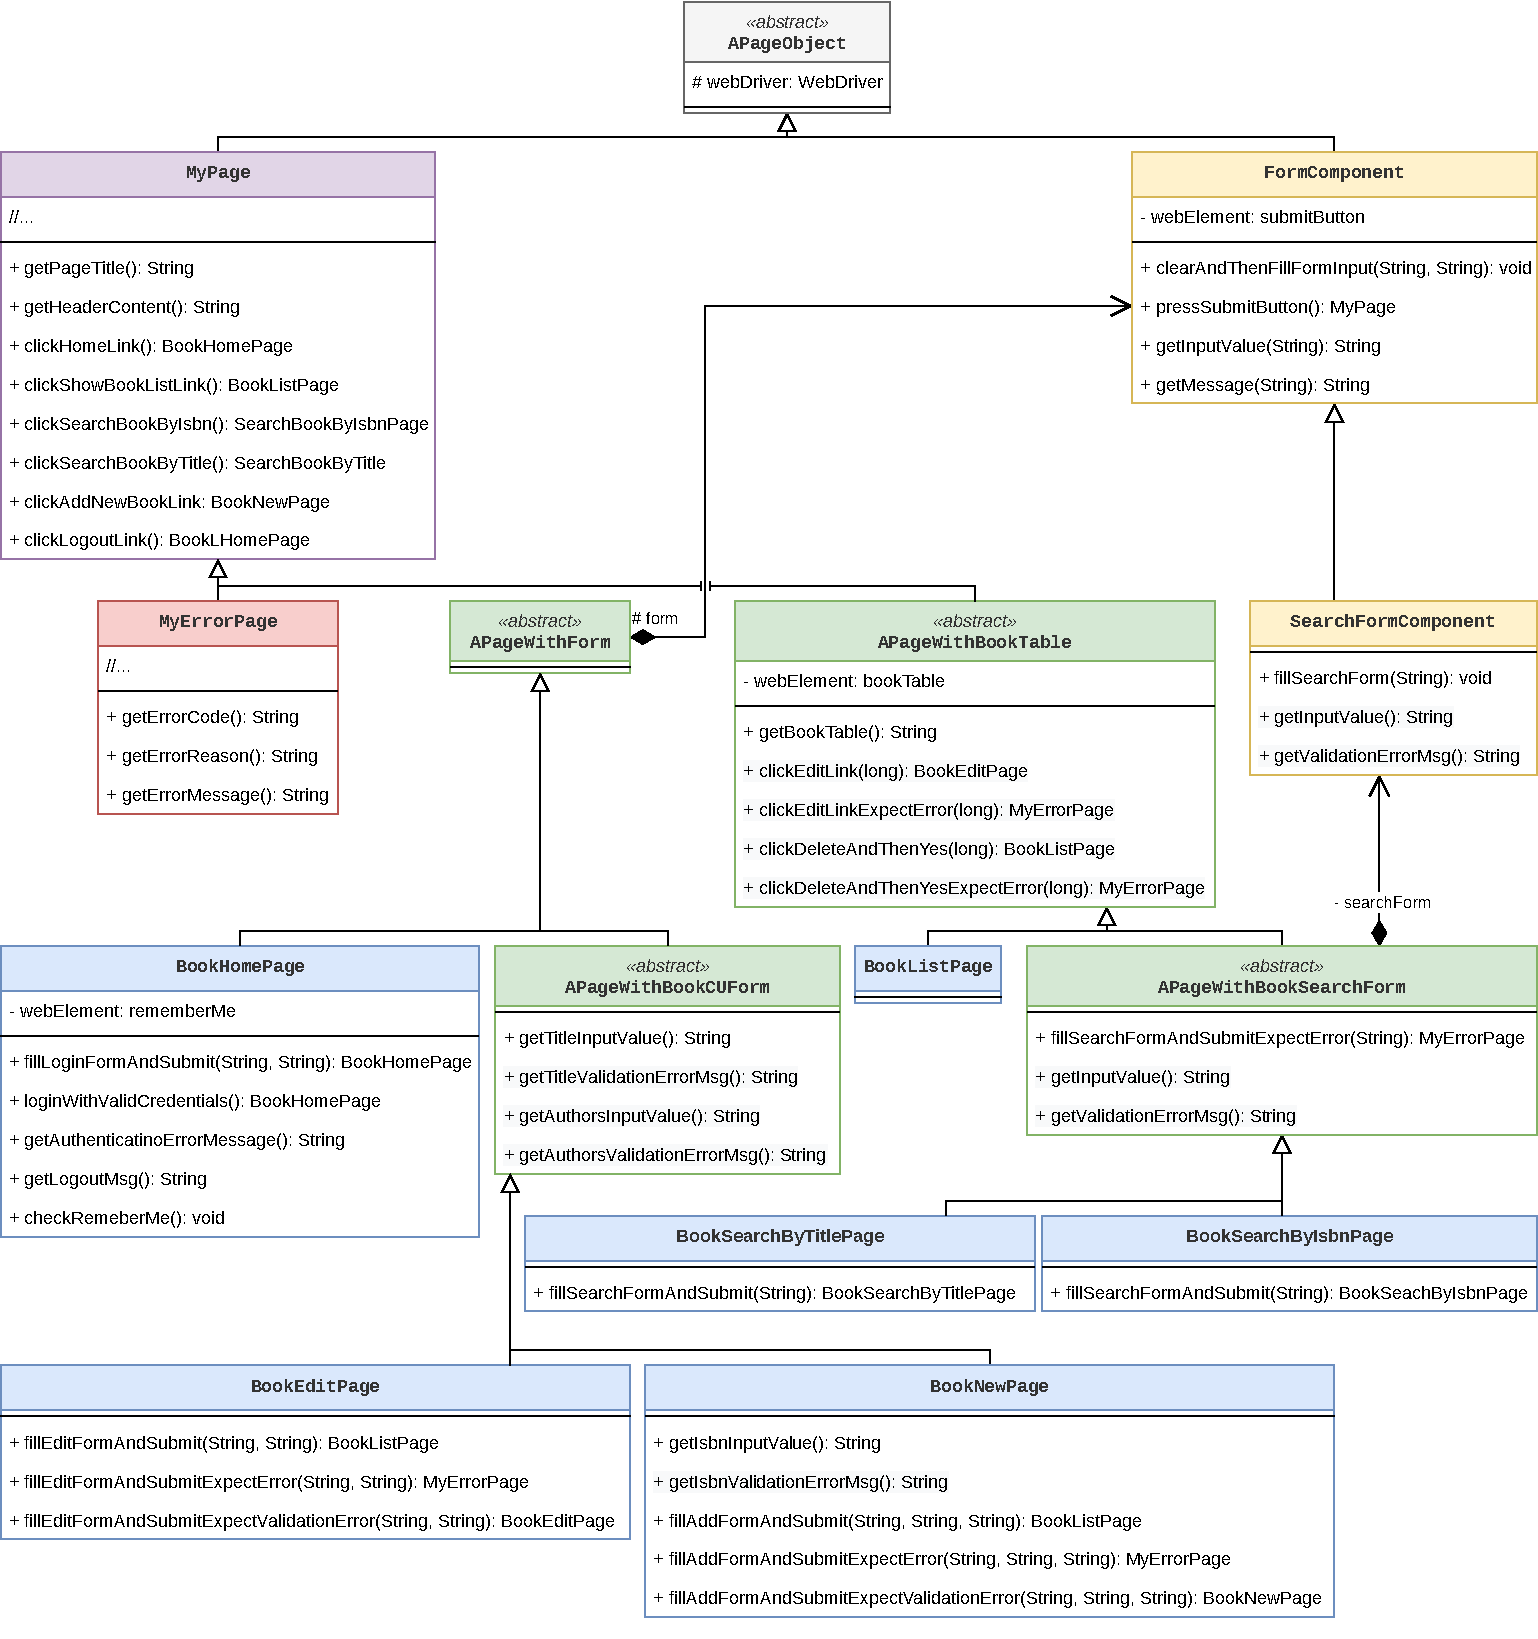
\includegraphics[width=\textwidth]{test/uml}
\caption[Figure example]{just a random figure example.}
\label{figure:uml}
\end{figure}

\section{Test table}

In \cref{table:esami} we see an example of a table.

\begin{table}[htbp]
\centering
\caption[Table example]{just a random table example.}
\label{table:esami}
\small
\begin{tabular}{lcc}
\toprule
\multicolumn{1}{c}{\textsc{Esami superati (12/12)}} & \textsc{Voto}&\textsc{CFU}\\ 
\midrule
Security and Network Management & 30-L & 6 \\
Sistemi Critici e Real Time & 28 & 6 \\
Ingegneria del Software & 30-L & 6 \\
Statistica Computazionale & 30-L & 9 \\
Interazione Uomo-Macchina & 30-L & 6 \\
Logica e Computazione Quantistica & 30-L & 6 \\
Progettazione e Analisi di Algoritmi & 30-L & 9 \\
Advanced Numerical Analysis & 30 & 6 \\
Analisi Quantitativa dei Sistemi & 29 & 9 \\
Security Engineering & 30-L & 9 \\
Advanced Techniques and Tools for Software Development & 30-L & 9 \\
Modelli di Sistemi Sequenziali e Concorrenti & 30-L & 9 \\
\bottomrule
\end{tabular}
\end{table}